\documentclass[headheight=4.5cm,
			   margin=2cm,
			   titlewidth=0.6,
			   sansserif,
			   firstcolor=color1,
			   secondcolor=color2,
			   logo=myLogo.png,
			   % footband=myFootBand.png
			  ]{TelecomNancy}

\definecolor{color1}{RGB}{100, 100, 100}
\definecolor{color2}{RGB}{220, 0, 0}
\usepackage{amsmath}
\usepackage{amssymb}
\usepackage{pifont}
\usepackage{tikz}
\usepackage{tabularx}
\usepackage{array}
\usepackage{booktabs}
\usepackage{multirow}
\usepackage{tabu}
\usepackage[UTF8]{ctex}

\begin{document}

	\coursetitle{椭圆及其标准方程\quad 学案}
	\courselevel{高中数学二年级}
	\courseyear{2018.12.12 Edited by Shine.Y}

	\globalinstructions[进入椭圆前的提示]
	{
		 古希腊的学者或是通过观察火山喷发,或是观察削尖的圆木桩,或是日晷的影子尖端轨迹,发现了“椭圆”这一优美的曲线,因为同研究“倍立方问题”有深刻的联系,椭圆进入了数学家的视野,之后一直是艺术、数学、天文学相互交融的重点。星汉灿烂,无数天体遵循开普勒定律绕着椭圆轨道运行,巴洛克时期的建筑师对于椭圆形建筑所爱尤甚。若是你有兴趣一探椭圆的究竟,请随我来.
	}

	\nextInstructions{\textbf{复习:圆的知识内容}}
			\nextQuestion{圆的定义是什么?}
			\nextQuestion{如何画一个圆?}
			\nextQuestion{圆的标准方程是什么?}

		\nextInstructions{\textbf{思考:} 平面内,到两个定点的距离之和等于定长的点的轨迹又是什么呢?
		}


	\nextExercise[什么是椭圆]{}

		\nextQuestion{\textbf{椭圆的定义:}平面内,到$\underline{\hspace{.5cm}}$个定点$F_1, F_2$ 的$\underline{\hspace{2cm}}$等于$\underline{\hspace{1cm}}$($\underline{\hspace{2cm}}$)的点的轨迹叫做椭圆.
		}

		\nextInstructions{\textbf{思考:} 平面内,到两定点$F_1, F_2$ 距离之和 等于 常数 的点$M$的轨迹都是椭圆吗?
		}
		若距离之和$(|MF_1| + |MF_2|)$ 为常数:
		\begin{itemize}
			\item 距离之和 \textbf{$>$} 焦距: 轨迹为$\underline{\hspace{2cm}}$
			\item 距离之和 \textbf{$=$} 焦距: 轨迹为$\underline{\hspace{2cm}}$
			\item 距离之和 \textbf{$<$} 焦距: 轨迹$\underline{\hspace{2cm}}$.
		\end{itemize}


	\nextExercise[椭圆的标准方程]{设定: 椭圆上的点到焦点的\textbf{距离之和}为"$\mathbf{2a}$",\textbf{焦距}为"$\mathbf{2c}$". (且$\mathbf{2a > 2c}$)}

		\nextQuestion{椭圆的标准方程的来源及化简方法.
		}
		\begin{minipage}{0.8\textwidth}
			椭圆上的点到焦点的距离之和 等于 定长 这样一个几何关系可以转换成一个怎样的数学语言呢?
		\end{minipage}
		\begin{minipage}{0.2\textwidth}
			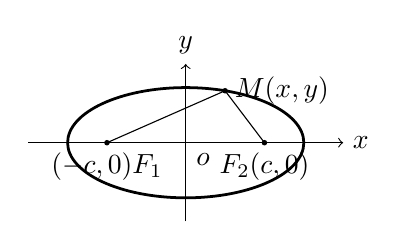
\begin{tikzpicture}
				\draw[->] (-2,0) -- (2,0)node[right]{$x$};
				\draw[->] (0,-1) -- (0,1)node[above]{$y$};
				\draw[line width=1pt] (0,0)node[below right]{$o$} ellipse [x radius=1.5cm, y radius=0.7cm];
				\fill (-1,0)node[below]{$(-c,0)F_1$} circle (1pt);
				\fill (1,0)node[below]{$F_2(c,0)$} circle (1pt);
				\fill (0.5,0.66)node[right]{$M(x,y)$} circle (1pt);
				\draw (-1,0)--(.5,.66);
				\draw (1,0)--(.5,.66);
			\end{tikzpicture}
		\end{minipage}

\newpage
		上式又该如何去化简呢?(\emph{提示:}要想使平方后的交叉项越来越简单,最好先移项,再平方哦. )\vspace{3cm}

		\nextQuestion{焦点在$x$轴上的椭圆的标准方程:$\underline{\hspace{3cm}}\mathbf{(a>b>0)}$
		\begin{minipage}{0.2\textwidth}
			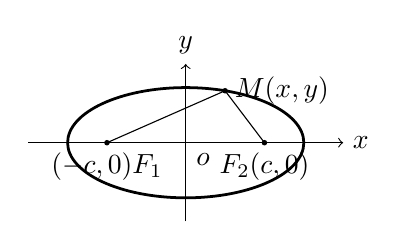
\begin{tikzpicture}
				\draw[->] (-2,0) -- (2,0)node[right]{$x$};
				\draw[->] (0,-1) -- (0,1)node[above]{$y$};
				\draw[line width=1pt] (0,0)node[below right]{$o$} ellipse [x radius=1.5cm, y radius=0.7cm];
				\fill (-1,0)node[below]{$(-c,0)F_1$} circle (1pt);
				\fill (1,0)node[below]{$F_2(c,0)$} circle (1pt);
				\fill (0.5,0.66)node[right]{$M(x,y)$} circle (1pt);
				\draw (-1,0)--(.5,.66);
				\draw (1,0)--(.5,.66);
			\end{tikzpicture}
		\end{minipage}
		}

		\nextQuestion{焦点在$y$轴上的椭圆的标准方程:$\underline{\hspace{3cm}}\mathbf{(a>b>0)}$
		\begin{minipage}{0.2\textwidth}
			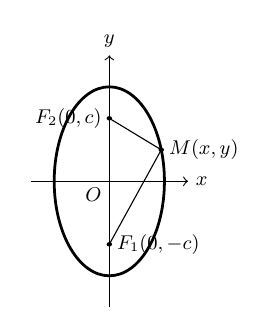
\begin{tikzpicture}[yscale=0.8]
				\tikzstyle{every node}=[font=\small,scale=0.8]
				\draw[->] (-1,0) -- (1,0)node[right]{$x$};
				\draw[->] (0,-2) -- (0,2)node[above]{$y$};
				\draw[line width=1pt] (0,0) ellipse [x radius=0.7cm, y radius=1.5cm];
				\fill (0,-1)node[right]{$F_1(0,-c)$} circle (1pt);
				\fill (0,1)node[left]{$F_2(0,c)$} circle (1pt);
				\fill (0.66,0.5)node[right]{$M(x,y)$} circle (1pt);
				\node[below=6pt,left] at (0,0) {$O$};
				\draw (0,-1)--(0.66,0.5);
				\draw (0,1)--(0.66,0.5);
			\end{tikzpicture}
		\end{minipage}
		}

		\textbf{特别注意:}
		\begin{itemize}
			\item 方程的形式:左边是两个分式的平方和,右边是"1";
			\item 三个参数$a,b,c$的关系:$\underline{\hspace{2.5cm}}$;
			\item 焦点跟着大数走("\textbf{比大小}").
		\end{itemize}


	\nextInstructions{\textbf{拓展练习:}求椭圆的标准方程}
		\nextQuestion{焦点坐标为$(0,-4), a=5$;} \vspace{1cm}
		\nextQuestion{焦点在$x$轴上,焦距等于4, 且经过点$P(3,-2 \sqrt{6})$;}\vspace{1cm}
		\nextQuestion{$a+c=10, a-c=4$.}\vspace{1cm}

	\nextInstructions{\textbf{课后作业:}《课时作业(八)》}

	\begin{minipage}{0.8\textwidth}
		\textbf{课后探索:}方程 $Ax^2 + By^2 =1$ 什么时候表示椭圆?什么时候表示焦点在 $x$ 轴上的椭圆?什么时候表示焦点在 $y$ 轴上的椭圆?能表示圆吗?

		\textbf{课后资料:}

		[1] 阿波罗尼斯奥:《圆锥曲线论》

		[2] 搜索引擎搜索关键词:丹德林双球
	\end{minipage}
	\begin{minipage}{0.2\textwidth}
		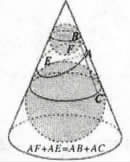
\includegraphics{e4.png}
	\end{minipage}

\end{document}
